% Original histogram data are unchanged. Only printed labels are covered and translated.
\definecolor{chfivecream}{RGB}{249,249,223}
\newcommand{\chfivediets}{%
\begin{tikzpicture}
\node[anchor=south west,inner sep=0] (image) at (0,0)
 {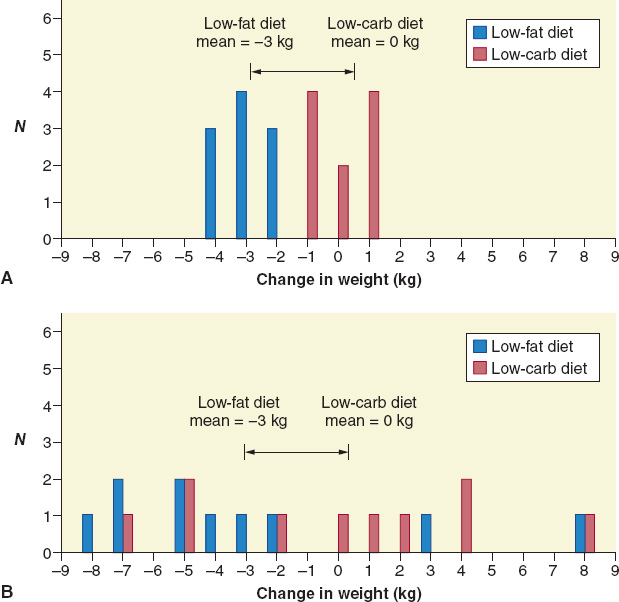
\includegraphics[width=15.3cm]{assets/ch05_diet_weight_loss.jpeg}};
\begin{scope}[x={(image.south east)},y={(image.north west)},font=\small]
\node[fill=chfivecream,inner sep=2pt,align=center,text width=2.55cm] at (.397,.945) {低脂饮食\\均值 $=-3$ kg};
\node[fill=chfivecream,inner sep=2pt,align=center,text width=2.55cm] at (.605,.945) {低碳水饮食\\均值 $=0$ kg};
\node[fill=chfivecream,inner sep=2pt,align=center,text width=2.55cm] at (.385,.313) {低脂饮食\\均值 $=-3$ kg};
\node[fill=chfivecream,inner sep=2pt,align=center,text width=2.55cm] at (.590,.313) {低碳水饮食\\均值 $=0$ kg};
\foreach \y in {.947,.426}{\node[fill=white,inner sep=1.5pt,align=left,text width=2.4cm,anchor=west] at (.789,\y) {低脂饮食};}
\foreach \y in {.909,.388}{\node[fill=white,inner sep=1.5pt,align=left,text width=2.4cm,anchor=west] at (.789,\y) {低碳水饮食};}
\foreach \y in {.535,.013}{\node[fill=white,inner sep=2pt,text width=6cm,align=center] at (.55,\y) {体重变化（kg）};}
\end{scope}
\end{tikzpicture}}
